\section{Introduction}\index{Eclipse!RCP!RAP}
The Eclipse Rich Ajax Platform (RAP)\index{Eclipse!RAP} allows Java
developers to build rich, Ajax-enabled Java applications that can be run on the
desktop or the web from a single code base.

RAP uses the Eclipse development model, plug-ins with the Eclipse workbench
extension points and a widget toolkit with SWT API. Which means that existing
Eclipse RCP applications can be run as web applications with just a few
modifications.

\begin{figure}[!htb]
  \begin{center}
    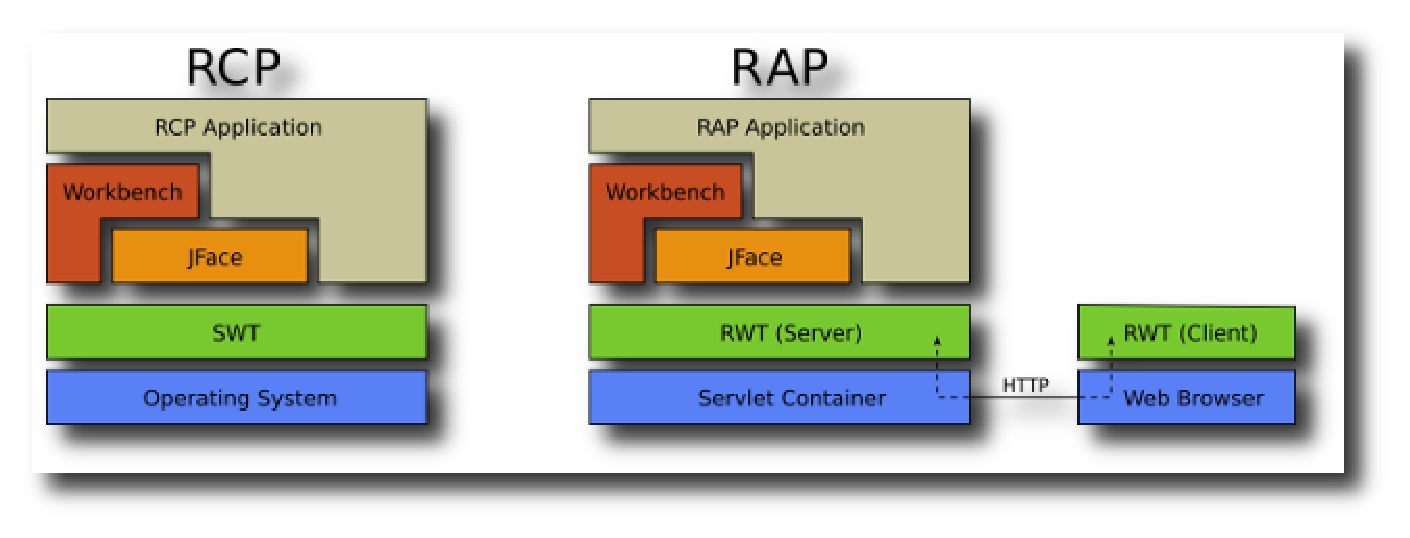
\includegraphics[scale=0.6]{Figures/Architecture_RAP.eps}
  \end{center}
  \caption{Eclipse RAP architecture}
  \label{Eclipse RAP architecture}
\end{figure}

\section{Advantages}\index{Eclipse!RAP!Inter browser compatibility}
\subsection{Inter browser compatibility}
RAP runs out of the box in all common web browsers. No browser add-ons are
required. The server part of RAP can be deployed on all Servlet Containers that
implement the Servlet API 2.3 through 3.0. This includes Tomcat, Jetty,
Glassfish, JBoss and WebSphere.

\subsection{Single sourcing}\index{Eclipse!RAP!Single sourcing}
A popular use case for RAP is the development of rich clients and web clients
from a single code base, also called "Single Sourcing". This allows Java and
Eclipse developers to reuse their existing skills. Furthermore, RAP maximizes
code reuse by including the largest-possible web-enabled subset of the Rich
Client Platform.
\\
\\
\emph{``Write once, run everywhere is the main objective of the
Java\texttrademark programming language ''}\cite{programming:java:spec}.
\\
\\
This holds true most of the time for running the same program on different
operating systems. But as technology evolves the Eclipse Foundations strives to
bring this slogan to a new level. Two technology projects, housed under the
Eclipse.org umbrella, namely RAP2 and eRCP3 , provide an alternative runtime
environment for RCP applications.

This means that the application - normally running as a desktop application on a
personal computer - can now be deployed to other runtime environments. For
example let us assume we have a ready to launch application based on RCP. By
switching the runtime from RCP to RAP, it becomes possible to launch the
application on an application server where clients ccan use the application with
a Web 2.0 centric interface on a browser.

There is no need for the user to install any further add-ons or plugins. In order
to achieve full compatibility between the platforms, many concepts implemented in
SWT \cite{eclipse:swt:wtoolkit} need to be adapted to other runtimes. These are
hidden behind the public API which remains synchronous across all runtime
projects. It may also be possible to change the structure of the application code
to fit the current runtime environment. Depending on the specific case, this may
be achievable through normal refactorings. The refactorings are not onerous and
generally lead to better quality bundles irrespective of the single-sourcing
requirement.

\subsection{Integration with BIRT}
\label{chap:RAP}
\index{Eclipse!RAP!Integration with BIRT}
\index{BIRT!Intergration in RAP applications}
Besides a rich user interaction many applications need to display a big amount of
data sets as diagrams or reports as part of their applications. In order to
bridge the gap the BIRT project was created as part of the eclipse ecosystem.

That BIRT integrates well with classic RCP applications is a well known fact. But
the need for rich internet applications is still growing. And here the RAP comes
into play. As a platform for developing Web 2.0 applications with the same
patterns as for RCP it paves the way for single sourcing applications running on
both platforms.
